\documentclass[11pt]{article}

% "review" gives line numbers and page numbers, as in the course reference.
% The \acl@anonymizefalse line below keeps author names visible.
% For a clean copy without line numbers, change "review" to "preprint".
\usepackage[review]{acl}
\makeatletter\acl@anonymizefalse\makeatother

\usepackage{times}
\usepackage{latexsym}
\usepackage[T1]{fontenc}
\usepackage[utf8]{inputenc}
\usepackage{microtype}
\usepackage{inconsolata}
\usepackage{graphicx}
\usepackage{booktabs}
\usepackage{array}

% The teaser figure below the authors needs room, so shrink the default title box.
\setlength\titlebox{3.3cm}

\title{Knowing When Not to Trust Depth:\\
A Learned Per-Pixel Confidence Head for Monocular Depth\\
in Adverse Driving Conditions}

\author{Nathan Aday, Alejandro Arteaga, Nathan Bao, Katherine Qiao, Varad Jaideep Tawde}

\begin{document}

\makeatletter
\g@addto@macro\@maketitle{%
  \begin{center}
    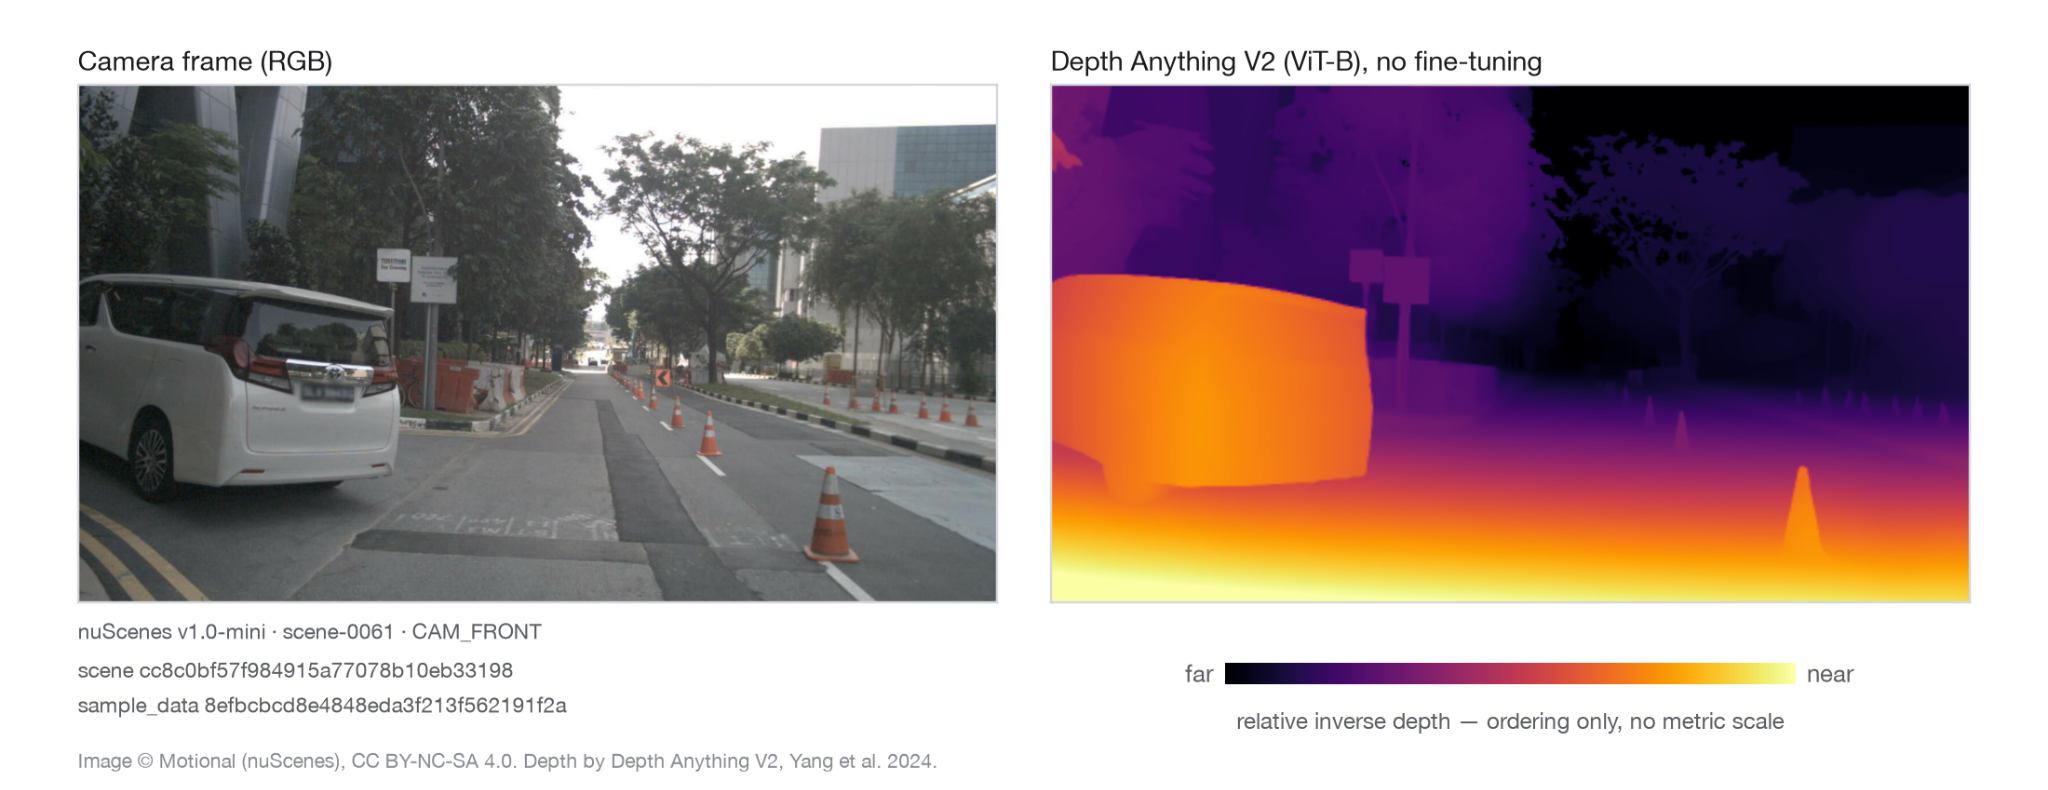
\includegraphics[width=0.75\textwidth]{figures/depth-anything-v2-example.png}
    \captionof{figure}{Example Depth Anything V2 output map.}
    \label{fig:example}
  \end{center}
  \vskip 0.05in}
\makeatother

\maketitle

\begin{abstract}
Monocular depth models such as Depth Anything V2 return a depth value for every pixel and no indication of which values to trust. A driving system places obstacles and plans a path from those values, but with no way to tell which are reliable. As depth degrades at night, through a rain-covered lens, or on object boundaries, we seek to add a metric of confidence to depth predictions. We train a small convolutional head that predicts, per pixel, whether the depth error exceeds a fixed threshold, based on sensor consensus between radar and LiDAR values for the same scene.
\end{abstract}

\section{Introduction}

Depth Anything and similar models supply depth to systems that have no depth sensor. They are used in driving, robotics, augmented reality, and 3D reconstruction, usually as a drop-in component. Every pixel gets a depth value and no measure of reliability: an estimate that is wrong by thirty percent looks exactly like one that is right.

In our own runs on nuScenes, Depth Anything V2 needs a per-image scale and shift fitted to lidar before its output is in meters. Even after that fit, the relative error is about ten percent by day and twenty percent at night. Nothing available at inference says which pixels carry that error.

This project trains a model to predict that error. A small convolutional head reads the frozen depth model's internal features along with three external inputs: temporal depth variance, a radar residual, and a radar validity mask. It outputs, per pixel, the probability that the depth there is wrong by more than a threshold. The head is the only component whose weights change.

The labels need no hand annotation. Projecting a lidar sweep into the camera image gives the true depth, and therefore the true error, at the pixels that receive a return. Under one percent of pixels carry a label, so the head learns from those scattered pixels and produces a dense map at inference. Lidar is present when we build the model and absent when the model runs, so the head must predict an error it cannot measure.

Driving data suits this task because a camera, a lidar, and a radar observe the same scene at the same time. Lidar gives the true depth and radar gives an independent range measurement in the same frame. The method is not specific to driving. Any system that consumes monocular depth has the same problem.

\subsection{Why it is useful}

The target application is adverse driving conditions. Night, rain on the lens, spray from other vehicles, and low sun are when camera depth is least reliable and when acting on a wrong depth costs the most. A confidence map lets a downstream consumer weight the depth, discard it, or fall back to another sensor. We can demonstrate two consumers: a reconstruction pipeline that ranks frames by mean confidence and keeps the highest-ranked ones, and an occupancy network that weights its camera-to-voxel lifting so unstable pixels contribute less.

\subsection{Why it is interesting}

Depth Anything is a large supervised model, used frozen, by people who did not train it and cannot retrain it. Whether confidence can be read from its features without retraining it is an open question.

Related work uses radar to improve the depth itself. HyDRa fuses radar features with image features before the depth head \citep{wolters2025hydra}, and LiCROcc distills lidar-camera knowledge into radar-camera scene completion \citep{ma2024licrocc}. We use radar to predict where the depth is wrong and leave the depth model untouched, so the output is a confidence map rather than a better depth map.

\section{Potential Solutions}

The proposed solution consists of a frozen monocular depth model followed by a lightweight learned confidence estimator. Rather than modifying the underlying depth prediction, the system is designed to predict where the existing depth estimates are likely to be unreliable. The confidence estimator combines information from the depth model itself with temporal and radar-based signals.

\subsection{Frozen Depth Backbone}

Depth Anything V2 \citep{yang2024depthanythingv2} will serve as the monocular depth backbone. The model will remain frozen during training, meaning that its parameters will not receive gradient updates. Each image will be passed through the model once to obtain its predicted depth and intermediate decoder features. These outputs can then be cached and reused while training the confidence model.

\subsection{Per-pixel Confidence Head}

A small convolutional network will be trained on top of the frozen depth backbone. Its input will consist of the decoder features produced by Depth Anything V2, the predicted depth map, temporal depth variance, the residual between predicted depth and radar range, and a radar validity mask. The network will output a single confidence channel at image resolution, representing the probability that the depth prediction at each pixel exceeds a fixed error threshold.

% A table* appears at the top of the page after the one where it is defined,
% so it is defined here to land at the top of the page with the Datasets section.
\begin{table*}[t]
  \centering
  \small
  \setlength{\tabcolsep}{4pt}
  \newcolumntype{P}[1]{>{\raggedright\arraybackslash}p{#1}}
  \begin{tabular}{@{}P{1.8cm} P{1.8cm} P{1.6cm} P{0.9cm} P{3.5cm} P{2.3cm} P{2.3cm}@{}}
    \toprule
    & \textbf{Cameras} & \textbf{Lidar} & \textbf{Radar} & \textbf{Size} & \textbf{Conditions} & \textbf{Role} \\
    \midrule
    nuScenes & 6 & 1, 32-beam & 5 & 1,000 scenes / 40k keyframes / 1.4M images & Day, night, rain & Training and evaluation \\
    STF / DENSE & 2 plus gated NIR & 2 & 1 & 12k on-road samples / 1.5k fog chamber & Fog, snow, rain & Candidate for heavier weather \\
    \bottomrule
  \end{tabular}
  \caption{Datasets that record lidar, camera sequences, radar, and condition labels together.}
  \label{tab:datasets}
\end{table*}

\section{Expected Outcomes}

The project produces one trained model, one measurement of how much of Depth Anything V2's error that model can predict, and two demonstrations of what a downstream consumer does with the prediction. Every result is reported separately for day, night, and rain on the nuScenes validation split.

\subsection{Confidence Map}

The primary outcome is the trained head and its sparsification curve: pixels are removed in order of predicted unreliability and the error of the remainder is plotted, bounded above by random removal and below by an oracle sorted on true lidar error. We report AUSE and AURG \citep{poggi2020uncertainty} against cheap baselines, random removal, raw temporal variance, flip-augmentation disagreement, and MC dropout where the checkpoint permits. We expect the largest margin over variance at night and in rain. If the head does not beat variance, the negative result is reported in the same table. Ablations without the radar channels and on decoder features alone decide what stays in the model.

\subsection{Stretch}

Once depth estimations can be trusted based on confidence, the next potential is to use these depth estimations for 3D occupancy grid construction. The 3D occupancy grid accuracy based on mIoU is a common benchmark for self driving perception, so measuring with and without the confidence head in the pipeline reveals another measure of effectiveness for the task.

\subsection{Deliverables}

Confidence maps per condition, one table (AUSE/AURG per method and condition), one plot (sparsification curves), and a repository.

\section{Datasets}

The method needs four things in the same recording: \textbf{lidar} projected into the image, the only source of error labels; \textbf{camera sequences}, since temporal variance needs neighboring frames; \textbf{calibrated radar}, which supplies two input channels; and \textbf{condition labels}, so results split by lighting and weather. Two datasets qualify (Table~\ref{tab:datasets}).

\subsection{nuScenes}

nuScenes \citep{caesar2020nuscenes} is the only public set with all four properties. It holds 1,000 driving scenes of 20 seconds each, recorded in Boston and Singapore. Annotation runs at 2~Hz and gives 40,000 keyframes; the unannotated camera sweeps between them supply the neighboring frames temporal variance needs. The official split is 700 scenes for training, 150 for validation, and 150 for test.

\subsection{STF / DENSE}

STF / DENSE \citep{bijelic2020seeing} covers weather nuScenes does not contain: about 12,000 on-road samples from more than 10,000~km in northern Europe, plus 1,500 recorded in a fog chamber. In the chamber, visibility is set rather than observed, so weather severity becomes a controlled variable.

\subsection{Also reviewed}

Zenseact ZOD is the backup: three lidars, 1,473 twenty-second sequences, Nordic weather, and a permissive license, but no radar, so two input channels have nothing to read. It becomes usable if the ablation shows radar was not carrying the head.

\section{Timeline}

\subsection{Weeks 1--3: Initiation and Review}

Task: Form the project team, clarify project goals, and survey related work on monocular depth confidence estimation, radar-camera fusion, and adverse-condition driving datasets.

\subsection{Weeks 4--6: Dataset Preparation}

Task: Download and preprocess nuScenes. Run Depth Anything V2 on the training split and cache decoder features and predicted depth. Project lidar sweeps into camera images to generate per-pixel error labels.

\subsection{Weeks 7--12: Model Development and Evaluation}

Task: Implement cheap baselines (temporal variance, flip-augmentation disagreement, random removal), train the convolutional confidence head, and evaluate using sparsification curves, AUSE, and AURG across day, night, and rain conditions.

\subsection{Dissemination}

Task: Compile results, stretch-goal experiments (frame selector, occupancy weighting) and analysis into a final report and repository.

\bibliography{references}

\end{document}
